\section{The \acl{MPM}}
\label{sec:mpm}
In this section, a description of the \ac{MPM} is provided. This work is
limited to the consideration of \ac{1D} and \ac{2D} \ac{NMR} data, and so both
the original \ac{1D} \ac{MPM} and its \ac{2D} analogue, the \ac{MMEMPM} is
provided. In theory, the method can be expanded to data with any number of
dimensions\cite{Yilmazer2006}, though given the typical size of \ac{NMR}
datasets, beyond \ac{2D} data the method is likely computationally intractable.

\subsection{1D Matrix Pencil Method}
\label{subsec:mpm}

\begin{remark}
    In contexts where \ac{1D} datasets are considered specifically, the
    redundant dimension index $^{(1)}$ will be neglected for conciseness.
\end{remark}
The \ac{MPM}, developed by Hua and Sarkar\cite{Hua1990,Hua1990b,Hua1991},
provides a route to extracting the signal poles of a \ac{1D} dataset, based on
the assumption that the number or oscillators $M$ is known.
To motivate how the \ac{MPM} works, first consider a dataset which is devoid of
noise, given by \cref{eq:x-alpha-z} with $D=1$:
\begin{equation}
    x_n(\bth) = \sumM \alpha_m^{\vphantom{n}} z_m^n,\\
\end{equation}
Consider the Hankel matrix $\Hx \in \mathbb{C}^{(N-L) \times (L+1)}$:
\begin{equation}
    \Hx =
    \begin{bmatrix}
        x_0 & x_1 & \cdots & x_L\\
        x_1 & x_2 & \cdots & x_{L+1}\\
        \vdots & \vdots & \ddots & \vdots\\
        x_{N-L-1} & x_{N-L} & \cdots & x_{N-1}
    \end{bmatrix}.
\end{equation}
This matrix comprises windowed segments of the FID, with each row comprising
the segment shifted to the right by one point relative to the row above.
$L \in \mathbb{N}$ is the \emph{pencil parameter}, which dictates the size of
each window. From $\Hx$, two matrices are defined, $\Hxone$ and $\Hxtwo$,
formed by the removal of the last or first column of $\Hx$, respectively:
\begin{subequations}
   \begin{gather}
        \Hxone =
        \begin{bmatrix}
            x_0 & x_1 & \cdots & x_{L-1} \\
            x_{1} & x_{2} & \cdots & x_{L} \\
            \vdots & \vdots & \ddots & \vdots\\
            x_{N-L-1} & x_{N-L} & \cdots & x_{N-2}\
        \end{bmatrix}, \\
        \Hxtwo =
        \begin{bmatrix}
            x_{1} & x_{2} & \cdots & x_{L} \\
            x_{2} & x_{3} & \cdots & x_{L+1} \\
            \vdots & \vdots & \ddots & \vdots\\
            x_{N-L} & x_{N-L+1} & \cdots & x_{N-1}\\
        \end{bmatrix}.
   \end{gather}
\end{subequations}
$\Hxone$ and  $\Hxtwo$ can be deconstructed into the following forms involving
matrices containing the $M$ signal poles and complex amplitudes that the data
comprises:
\begin{subequations}
   \begin{gather}
       \Hxone = \symbf{Z}_{\text{L}} \symbf{A} \symbf{Z}_{\text{R}},\\
       \Hxtwo = \symbf{Z}_{\text{L}} \symbf{A} \symbf{Z}_{\text{D}} \symbf{Z}_{\text{R}},\\
       \mathbb{C}^{\left(\None - \Lone\right) \times M} \ni
       \symbf{Z}_{\text{L}} =
       \begin{bmatrix}
           \symbf{1} &
           \symbf{z} &
           \symbf{z}^2 &
           \cdots &
           \symbf{z}^{N-L-1}
        \end{bmatrix}\T,\\
        \mathbb{C}^{M \times L} \ni
        \symbf{Z}_{\text{R}} =
           \begin{bmatrix}
               \symbf{1} & \symbf{z} & {\symbf{z}}^{2} & \cdots & {\symbf{z}}^{L-1}
           \end{bmatrix} ,\\
        \mathbb{C}^{M \times M} \ni
        \symbf{Z}_{\text{D}} = \diag\left(\symbf{z}\right), \label{eq:ZD}\\
        \mathbb{C}^{M \times M} \ni
        \symbf{A} = \diag\left(\symbf{\alpha}\right),\label{eq:A}\\
        \symbf{\alpha} =
        \begin{bmatrix}
            \alpha_1 & \alpha_2 & \cdots & \alpha_M
        \end{bmatrix}\T,\\
        \symbf{z} =
        \begin{bmatrix}
            z_1 & z_2 & \cdots & z_M
        \end{bmatrix}\T.
   \end{gather}%
    \label{eq:HX-decomp}%
\end{subequations}%
The \emph{matrix pencil} $\Hxtwo - \lambda\Hxone$, with $\lambda \in
\mathbb{C}$, can therefore be expressed as
\begin{equation}
    \Hxtwo - \lambda \Hxone = \symbf{Z}_{\text{L}} \symbf{A} \left(
        \symbf{Z}_{\text{D}} - \lambda \symbf{I}_M
    \right) \symbf{Z}_{\text{R}},
\end{equation}
where $\symbf{I}_M \in \mathbb{C}^{M \times M}$ is the identity matrix.
Assuming that the following condition is met:
\begin{equation}
    M \leq L \leq N - M,\label{eq:pencil_condition}
\end{equation}
the rank of the matrix pencil will be $M$. \cref{eq:pencil_condition}
must be obeyed to ensure that both the number of rows and columns of the matrix
pencil are at least $M$. Now consider the case when the scalar $\lambda$ is
equal to one of the signal poles i.e.  $\lambda = z_m\ \forall m \in
\lbrace 1, \cdots, M \rbrace$. The element $[\symbf{Z}_{\text{D}} -
\lambda \symbf{I}_M]_{m,m}$ will be set to $0$, which will lead to the
determinant of the matrix pencil being $0$. The eigenvalues of the matrix
pencil are the solution of the so-called \emph{generalised eigenvalue problem},
and are defined as\cite[Section 7.7]{Golub2013}
\begin{equation}
    \symbf{z} = \left\lbrace
        z \in \mathbb{C} : \det\left(\Hxtwo - z \Hxone\right) = 0
    \right\rbrace
\end{equation}
One means of finding the signal poles is by finding the eigenvalues of the
matrix $\Hxone^+ \Hxtwo^{\vphantom{+}}$. Deriving the corresponding complex
amplitudes can then be achieved by solving the set of linear equations%
\begin{subequations}%
    \begin{gather}
        \symbf{\alpha} = \symbf{Z}^+ \symbf{x},\\
        \symbf{Z} =
        \begin{bmatrix}
            \symbf{1} &
            {\symbf{z}} &
            {\symbf{z}}^2 &
            \cdots &
            {\symbf{z}}^{N-1}
        \end{bmatrix}\T.
    \end{gather}%
    \label{eq:comp-amps}%
\end{subequations}%
Extraction of the amplitudes, phases, frequencies, and damping factors from the
signal poles and complex amplitudes can then take place:%
\begin{subequations}%
    \begin{gather}
        \symbf{a} = \left \lvert \symbf{\alpha} \right \rvert,\\
        \symbf{\phi} = \arctan \left(\frac{\Im (\symbf{\alpha})}{\Re(\symbf{\alpha})}\right),\\
        \symbf{f} = \frac{\fsw}{2 \pi} \Im\left(\ln \symbf{z} \right) + \foff,\label{eq:poles-to-f}\\
        \symbf{\eta} = -\fsw \Re\left(\ln \symbf{z}\right).
    \end{gather}
\end{subequations}

Noise corruption complicates the process of
determining the $M$ signal poles, as $\Hy$\,---\,$\Hx$'s equivalent with
elements replaced by the noisy data $\symbf{y}$\,---\, is likely to be
full-rank, given by $\min(N - L, L + 1)$. To minimise the influence of noise on
the estimated signal poles, it is necessary to
generate a rank-reduced matrix $\Hytilde$. By employing the \ac{EYM}
theorem\cite[Section~2.2]{Golub2013}, an appropriate matrix is can be obtained
through \ac{SVD} (see \cref{subsec:linear-algebra}):
\begin{subequations}
    \begin{gather}
    \Hytilde =
        \symbf{U}_M^{\vphantom{\dagger}}
        \symbf{\Sigma}_M^{\vphantom{\dagger}}
        \symbf{V}_M^{\dagger},\\
    \mathbb{C}^{(\None - \Lone) \times M} \ni
        \symbf{U}_M^{\vphantom{\dagger}} =
        \begin{bmatrix}
            \symbf{u}_1 &
            \symbf{u}_2 &
            \cdots &
            \symbf{u}_M
        \end{bmatrix},\\
    \mathbb{C}^{(\Lone + 1) \times M} \ni
        \symbf{V}_M^{\vphantom{\dagger}} =
        \begin{bmatrix}
            \symbf{v}_1 &
            \symbf{v}_2 &
            \cdots &
            \symbf{v}_M
        \end{bmatrix},\\
    \mathbb{C}^{M \times M} \ni
        \symbf{\Sigma}_M^{\vphantom{\dagger}} =
        \diag \left( \sigma_1, \sigma_2, \cdots, \sigma_M \right).
    \end{gather}
\end{subequations}
$\sigma_m$ is the $m$\textsuperscript{th} largest singular value of $\Hy$,
while $\symbf{u}_m \in \mathbb{C}^{N - L}$ and $\symbf{v}_m \in
\mathbb{C}^{L+1}$ are the corresponding left and right singular vectors,
respectively. The \ac{EYM} theorem proves that $\Hytilde$ is the closest matrix
of rank $M$ to $\Hy$ in a Frobenius norm sense, i.e.
\begin{equation}
    \Hytilde = \argmin_{\symbf{A}:\ \rank(\symbf{A}) = M} \left \lVert \symbf{A} - \Hy \right \rVert.
\end{equation}
With a rank-reduced matrix produced from the noisy matrix, the signal poles can
then be derived from the eigenvalues of $\Hytildeone^+
\Hytildetwo^{\vphantom{+}}$, where $\Hytildeone$ and $\Hytildetwo$ have the
same relation to $\Hytilde$ as  $\Hxone$ and  $\Hxtwo$ do to  $\Hx$. As a
less expensive alternative, the same result can be achieved by
computing the eigenvalues of $\symbf{V}_{M1}^+\symbf{V}_{M2}^{\vphantom{+}}$,
with
\begin{subequations}
    \begin{gather}
        \symbf{V}_{M1} =
        \begin{bmatrix}
            \symbf{v}_1 & \symbf{v}_2 & \cdots & \symbf{v}_{M-1}
        \end{bmatrix},\\
        \symbf{V}_{M2} =
        \begin{bmatrix}
            \symbf{v}_2 & \symbf{v}_3 & \cdots & \symbf{v}_{M}
        \end{bmatrix}.
    \end{gather}
\end{subequations}
\cref{alg:mpm} provides a pseudo-code description of the \ac{MPM}, while
\cref{lst:mpm} outlines a \Python implementation of it. For optimal
results, the pencil parameter should adhere to $\lfloor \nicefrac{N}{3} \rfloor
\leq L \leq \lfloor\nicefrac{2N}{3}\rfloor$\cite{Hua1990}. In this work,
$\lfloor\nicefrac{N}{3}\rfloor$ is always used, primarily since the computational
complexity of the method is at a maximum when $L = \nicefrac{N}{2}$\footnote{
    With $L = \lfloor\nicefrac{N}{2}\rfloor$, the matrix
    $\Hy$ is at its most ``square'' i.e. the number of rows
    and columns are at their most similar. Matrices which are more
    square will increase the demands on computing the \ac{SVD}, with a
    complexity $\mathcal{O}(\min(L+1,N-L+1)^2 \times \max(L+1,N-L+1))$.
}.

\begin{algorithm}
    \caption[
        The \acl{MPM}, with the optional prediction of model order using the
        \acl{MDL}.
    ]
    {
        The \acs{MPM}, with the optional prediction of model order using the
        \acs{MDL} if $M$ is set to $0$.
    }\label{alg:mpm}
    \begin{algorithmic}[1]
        \Procedure{MPM}{$\by \in \mathbb{C}^{N}, \fsw \in \mathbb{R}_{>0}, \foff \in \mathbb{R}, M \in \mathbb{N}_0$}
            \State $L \gets \left\lfloor \nicefrac{N}{3} \right\rfloor$;
            \State $\symbf{H}_{\symbf{y}} \gets
                \begin{bmatrix}
                    y_{0} & y_{1} & \cdots & y_{L}\\
                    y_{1} & y_{2} & \cdots & y_{L+1}\\
                    \vdots & \vdots & \ddots & \vdots\\
                    y_{N-L-1} & y_{N-L} & \cdots & y_{N-1}\\
                \end{bmatrix}
            $;
            \State $\symbf{U}, \symbf{\sigma}, \symbf{V} \gets
            \SVD(\symbf{H}_{\symbf{y}})$;
            \If {$M = 0$}
                \State $M \gets \operatorname{MDL}(\symbf{\sigma}, L, N)$;
            \EndIf
            \State $\symbf{V}_{M1}, \symbf{V}_{M2} \gets
            \begin{bmatrix}
                \symbf{v}_1 & \symbf{v}_2 & \cdots & \symbf{v}_{M-1}
            \end{bmatrix},
            \begin{bmatrix}
                \symbf{v}_2 & \symbf{v}_3 & \cdots & \symbf{v}_{M}
            \end{bmatrix}
            $;
            \State $\symbf{z} \gets \textsc{Eigenvalues}\left(\symbf{V}_{M1}^+ \symbf{V}_{M2}^{\vphantom{+}}\right)$;
            \State $\symbf{Z} \gets
                \begin{bmatrix}
                    \symbf{1} & \symbf{z} & {\symbf{z}}^2 & \cdots & {\symbf{z}}^{N}
                \end{bmatrix}\T
            $;
            \State $\bdalpha \gets \symbf{Z}^+ \by$;
            \State $
                \symbf{a}, \symbf{\phi} \gets \left\lvert\symbf{\alpha}\right\rvert,
                \arctan \left(\frac{\Im(\symbf{\alpha})}{\Re(\symbf{\alpha})}\right)
                $;
            \State $\symbf{f}, \symbf{\eta} \gets \frac{\fsw}{2\pi} \Im \left( \ln \symbf{z} \right) + \foff,
                -\fsw \Re \left( \ln \symbf{z} \right)
            $;
            \If {$\symbf{\eta}$ contains negative values}
            \Comment{Purge any oscillators with negative damping}
                \State Remove these from $\symbf{\eta}$, and remove the
                corresponding values from
                $\symbf{a}$, $\symbf{\phi}$, and $\symbf{f}$;
            \EndIf
            \State $\bthzero \gets
                \begin{bmatrix}
                    \symbf{a}\T &
                    \symbf{\phi}\T &
                    \symbf{f}\T &
                    \symbf{\eta}\T
                \end{bmatrix}\T
            $;
            \State \textbf{return} $\bthzero$;
        \EndProcedure
        \Statex
        \Procedure{MDL}{$\symbf{\sigma} \in \mathbb{R}^{L+1}, L \in \mathbb{N}, N \in \mathbb{N}$}
            \For {$k = 0, \cdots, L$}
                \State $\operatorname{MDL}_k \gets
                -\ln\left(
                    \frac
                    {\prod_{r=k}^{L-1} \sigma_{r+1}^{\nicefrac{1}{L-k}}}
                    {\frac{1}{L-k} \sum_{r=k}^{L-1} \sigma_{r+1}}
                \right)^{(L-k)N}
                + \frac{1}{2}k(2L - k)\ln N
                $;
                \If {$k > 0$ \textbf{and} $\operatorname{MDL}_k > \operatorname{MDL}_{k-1}$}
                    \State $M \gets k-1$;
                    \State \textbf{break};
                \EndIf
            \EndFor
            \State \textbf{return} $M$;
        \EndProcedure
    \end{algorithmic}
\end{algorithm}


\subsection{2D Matrix Enhancement and Matrix Pencil Method}
\label{subsec:mmempm}
The \ac{MPM} was extended for the consideration of \ac{2D} data by Hua with the
\acfi{MEMPM}\cite{Hua1992}. The method centers around the enhanced matrix $\EY
\in \mathbb{C}^{\Lone \Ltwo \times (\None - \Lone + 1)(\Ntwo - \Ltwo + 1)}$,
a block Hankel matrix of the form
\begin{subequations}
    \begin{gather}
        \EY =
        \begin{bmatrix}
            \symbf{H}_{\symbf{y},0} & \symbf{H}_{\symbf{y},1} & \cdots & \symbf{H}_{\symbf{y},\None - \Lone} \\
            \symbf{H}_{\symbf{y},1} & \symbf{H}_{\symbf{y},2} & \cdots & \symbf{H}_{\symbf{y},\None - \Lone + 1} \\
            \vdots & \vdots & \ddots & \vdots \\
            \symbf{H}_{\symbf{y},\Lone - 1} & \symbf{H}_{\symbf{y},\Lone} & \cdots & \symbf{H}_{\symbf{y},\None - 1}
        \end{bmatrix}, \\
        \def\arraystretch{1.3}
        \symbf{H}_{\symbf{y},\none} =
        \begin{bmatrix}
            y_{ \none, 0 } & y_{ \none, 1 } & \cdots & y_{ \none, \Ntwo - \Ltwo } \\
            y_{ \none, 1 } & y_{ \none, 2 } & \cdots & y_{ \none, \Ntwo - \Ltwo + 1 } \\
            \vdots & \vdots & \ddots & \vdots \\
            y_{ \none, \Ltwo - 1 } & y_{ \none, \Ltwo } & \cdots & y_{ \none, \Ntwo - 1 }
        \end{bmatrix}.
    \end{gather}
\end{subequations}
In a similar fashion to \cref{eq:HX-decomp},
$\symbf{H}_{\symbf{x},\none}$, the noiseless equivalent to
$\symbf{H}_{\symbf{y},\none}$, can be expressed as
\begin{equation}
    \symbf{H}_{\symbf{x},\none} =
        \symbf{Z}^{(2)}_{\text{L}}
        \symbf{A}
        {\symbf{Z}^{(1)}_{\text{D}}}^{\none}
        \symbf{Z}^{(2)}_{\text{R}}.
\end{equation}
This then enables the noiseless enhanced matrix to be expressed as
\begin{subequations}
    \begin{gather}
        \symbf{E}_{\symbf{X}} =
        \symbf{E}_{\text{L}}
        \symbf{A}
        \symbf{E}_{\text{R}},\\
        \mathbb{C}^{\Lone \Ltwo \times M} \ni
        \symbf{E}_{\text{L}} =
        \begin{bmatrix}
            \symbf{Z}^{(2)}_{\text{L}} \\
            \symbf{Z}^{(2)}_{\text{L}} \symbf{Z}^{(1)}_{\text{D}} \\
            \vdots \\
            \symbf{Z}^{(2)}_{\text{L}} {\symbf{Z}^{(1)}_{\text{D}}}^{\Lone - 1} \\
        \end{bmatrix},\label{eq:EL}\\
        \mathbb{C}^{M \times \left(\None - \Lone + 1\right)\left(\Ntwo - \Ltwo + 1\right)} \ni
        \symbf{E}_{\text{R}} =
        \begin{bmatrix}
            \symbf{Z}^{(2)}_{\text{R}} &
            \symbf{Z}^{(1)}_{\text{D}} \symbf{Z}^{(2)}_{\text{R}} &
            \cdots &
            {\symbf{Z}^{(1)}_{\text{D}}}^{\None - \Lone} \symbf{Z}^{(2)}_{\text{R}} \\
        \end{bmatrix}.
    \end{gather}
\end{subequations}
As was the case in the \ac{1D} \ac{MPM}, \ac{SVD} can be utilised to generate a
filtered matrix $\EYtilde$ with its rank reducd to $M$, in accordance witht he
\ac{EYM} theorem:
\begin{equation}
    \EYtilde =
        \symbf{U}_M^{\vphantom{\dagger}}
        \symbf{\Sigma}_M^{\vphantom{\dagger}}
        \symbf{V}_M^{\dagger}
\end{equation}
Due to the large size of the enhanced matrix, a vast improvement
in the speed of the \ac{MEMPM} can be realised when, rather than compute the
\ac{SVD} in its entirety, a \emph{truncated} \ac{SVD} is computed, in
which only the first $M$ components of the \ac{SVD} are
determined\cite{Baglama2005}.

If the conditions $\Nd - L^{(d)} + 1 \geq M\ \forall d \in \lbrace 1, 2
\rbrace$ are met, $\range\left(\symbf{U}_M\right) =
\range\left(\symbf{E}_{\text{L}}\right)$. This implies that there is some
nonsingular matrix $\symbf{T} \in \mathbb{C}^{M \times M}$ such that
\begin{equation}
    \symbf{U}_M = \symbf{E}_{\text{L}} \symbf{T}.
\end{equation}
Now consider the following two matrices:
\begin{subequations}
    \begin{gather}
        \symbf{U}_{M1} = \symbf{E}^{\vphantom{(1)}}_{\text{L}1} \symbf{T},\\
        \symbf{U}_{M2} = \symbf{E}^{\vphantom{(1)}}_{\text{L}1} \symbf{Z}^{(1)}_{\text{D}} \symbf{T},\\
        \mathbb{C}^{\Lone \left(\Ltwo - 1\right) \times M} \ni
        \symbf{E}_{\text{L}1} =
        \begin{bmatrix}
            \symbf{Z}^{(2)}_{\text{L}} \\
            \symbf{Z}^{(2)}_{\text{L}} \symbf{Z}^{(1)}_{\text{D}} \\
            \vdots \\
            \symbf{Z}^{(2)}_{\text{L}} {\symbf{Z}^{(1)}_{\text{D}}}^{\Lone - 2}
        \end{bmatrix}.
    \end{gather}
\end{subequations}
$\symbf{U}_{M1}$ and $\symbf{U}_{M2}$ correspond the $\symbf{U}_M$ with the
last and first $\Ltwo$ rows removed, respectively. The matrix pencil for
$\symbf{U}_{M1}$ and $\symbf{U}_{M2}$ can be expressed as
\begin{equation}
    \symbf{U}_{M1} - \lambda \symbf{U}_{M2} =
    \symbf{E}_{\text{L}1} \left( \symbf{Z}^{(1)}_{\text{D}} - \lambda \symbf{I}_M \right) \symbf{T}.
\end{equation}
As seen previously, this matrix structure implies that the elements of
$\bdzone$ are the solutions to the generalised eigenvalue problem, such that
they are the eigenvalues of $\symbf{U}_{M1}^{+} \symbf{U}_{M2}^{\vphantom{+}}$.

To extract the signal poles in the other dimension, $\bdztwo$, the permutation
matrix $\symbf{P} \in \mathbb{R}^{\Lone \Ltwo \times \Lone \Ltwo}$ is defined:
\begin{equation}
    \symbf{P} =
    {\small
    \begin{bmatrix}
        \symbf{e}\left(1\right) \\
        \symbf{e}\left(1 + \Ltwo\right) \\
        \vdots \\
        \symbf{e}\left(1 + \left(\Lone - 1\right)\Ltwo\right) \\
        \symbf{e}\left(2\right) \\
        \symbf{e}\left(2 + \Ltwo\right) \\
        \vdots \\
        \symbf{e}\left(2 + \left(\Lone - 1\right)\Ltwo\right) \\
        \vdots \\
        \vdots \\
        \symbf{e}\left(\Ltwo\right) \\
        \symbf{e}\left(2\Ltwo\right) \\
        \vdots \\
        \symbf{e}\left(\Lone \Ltwo\right) \\
    \end{bmatrix}.
    }
\end{equation}
$\symbf{e}\left(i\right) \in \mathbb{R}^{\Lone \Ltwo}$ corresponds to a unit row
vector comprising zeros except for $e_i = 1$.
Multiplying $\symbf{E}_{\text{L}}$ by the permutation matrix leads to a matrix
in which the roles of the two sets of signal poles are effectively swapped:
\begin{equation}
    \symbf{E}_{\text{LP}} \coloneq \symbf{P} \symbf{E}_{\text{L}} =
    \begin{bmatrix}
        \symbf{Z}^{(1)}_{\text{L}} \\
        \symbf{Z}^{(1)}_{\text{L}} \symbf{Z}^{(2)}_{\text{D}} \\
        \vdots \\
        \symbf{Z}^{(1)}_{\text{L}} {\symbf{Z}^{(2)}_{\text{D}}}^{\Ltwo - 1} \\
    \end{bmatrix}.\label{eq:ELP}
\end{equation}
Note the similarity of \cref{eq:ELP} with \cref{eq:EL}, which
implies that with the same reasoning as above, $\bdztwo$ can be derived
by extracting the eigenvalues of $\symbf{U}_{M\text{P}1}^+
\symbf{U}_{M\text{P}2}^{\vphantom{+}}$, where $\symbf{U}_{M\text{P}1}$ and
$\symbf{U}_{M\text{P}2}$ correspond to $\symbf{P} \symbf{U}_M$
with the last and first $\Lone$ rows removed, respectively.

\begin{figure}
    \centering
    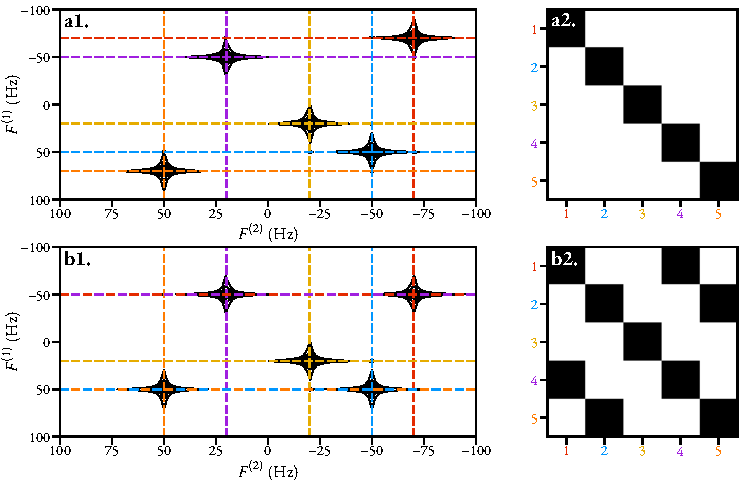
\includegraphics{mmempm_poles/mmempm_poles.pdf}
    \caption[
        A comparison of the structure of the matrix $\symbf{G}$ from the
        \acs{MMEMPM}, for the cases of an \acs{FID} with distinct signal poles
        in $\Fone$ and one with repeated signal poles
    ]{
        A comparison of the structure of the matrix $\symbf{G}$ from the
        \acs{MMEMPM}, for the cases of an \acs{FID} with \textbf{a.} distinct
        signal poles in $\Fone$ and \textbf{b.} one with repeated signal poles.
        \textbf{a1.} Magntiude-mode spectrum of a hypercomplex \ac{2D}
        \ac{FID}, with $M=5$, and all indirect-dimension frequencies having
        distinct values.
        \textbf{b1.} An equivalent spectrum with two pairs of the $5$
        indirect-dimension frequencies being identical ($\lbrace 1, 4 \rbrace$
        and  $\lbrace 2, 5 \rbrace$).
        \textbf{a2.} A representation of the matrix
        $\lvert \symbf{G} \rvert$ for the dataset depicted in a1. All values
        which are greater than \num{1e-10} are coloured black, while those that
        are less than \num{1e-10} are white.
        \textbf{b2.} An analogous representation for the dataset in b1. Note
        that $\symbf{G}$ is no longer diagonal, but possesses non-zero
        off-diagonal elements in agreement with signals with equivalent poles.
        With an appropriate re-ordering of the rows and columns (i.e. swapping
        the rows and columns of 2 and 4), this could be recast as a
        block-diagonal matrix featuring 3 blocks, one which is $1 \times 1$,
        and two which are  $2 \times 2$.
    }
    \label{fig:mmempm-poles}
\end{figure}
In the original account on the \ac{MEMPM}, the final stage involved employing a
pairing algorithm in order to assign the uncorrelated signal poles in $\bdzone$
with $\bdztwo$\cite{Hua1992}. The \emph{modified} \ac{MEMPM} (\acs{MMEMPM}) was
developed in order to overcome two issues with the pairing algorithm: (a) it is
computationally expensive (b) it is prone to return incorrect
pairings\cite{Chen2007}.
The procedure for extracting the paired poles differs slightly depending on
whether in the first dimension, all the signal poles in $\symbf{z}^{(1)}$ are
distinct or not.
As well as the eigenvalues of
$\symbf{U}^{+}_{M1}\symbf{U}_{M2}^{\vphantom{+}}$, the \ac{MMEMPM} requires
the corresponding eigenvectors too, contained in the matrix
$\symbf{W}^{(1)}$. Assuming that there are no repeated poles in
$\bdzone$\footnote{
    For the purposes of \ac{FID} estimation, it is deemed that a given pair
    $i,j \in \lbrace 1, \cdots, M \rbrace$ of poles is repeated if their
    frequencies satisfy $\lvert \fone_i - \fone_j \rvert <
    \nicefrac{\fswone}{\None}$ (recall \cref{eq:poles-to-f}, which states the
    relationship between a signal pole and its frequency).
    \label{fn:similar-freqs}
}, the following holds:
\begin{equation}
    \bdZtwo_{\text{D}} \equiv \symbf{G} =
        {\symbf{W}^{(1)}}^{-1}
        \symbf{U}_{M\text{P}1}^+
        \symbf{U}_{M\text{P}2}^{\vphantom{+}}
        \symbf{W}^{(1)},
\end{equation}
such that the second dimension signal poles are determined with $\bdztwo =
\diag(\symbf{G})$ (see panel a of \cref{fig:mmempm-poles}).
If some some values in $\bdzone$ are repeated, the matrix $\symbf{G}$ is
no longer diagonal, but instead and can be expressed as block-diagonal;
assuming there are $R < M$ unique signal poles, $\symbf{G}$ has the form
\begin{equation}
    \symbf{G} =
    \begin{bmatrix}
        \symbf{G}_1 & \symbf{0} & \cdots & \symbf{0} \\
        \symbf{0} & \symbf{G}_2 & \cdots & \symbf{0} \\
        \vdots & \vdots & \ddots & \vdots \\
        \symbf{0} & \symbf{0} & \cdots & \symbf{G}_R
    \end{bmatrix}
    \label{eq:block-G}
\end{equation}
where $\symbf{G}_r \in \mathbb{C}^{h_r \times h_r}$ is a sub-matrix corresponding
to the $r$\textsuperscript{th} unique signal pole with multiplicity $h_r$ (see
panel b of \cref{fig:mmempm-poles}). Note that $\sum_{r=1}^R h_r = M$. When
$h_r > 1$, the subset of poles $\bdztwo_r$ are determined by computing the
eigenvalues of the matrix $\symbf{G}_r$

See \cref{alg:mmempm} for a pseudo-code outline, and \cref{lst:mmempm} for a
\Python implementation of the \ac{MMEMPM}.

\subsection{Model Order Selection}
\label{subsec:model-order}
The \ac{MPM} and \ac{MMEMPM} operate under the assumption that the model order
$M$ is known, or at least has been predicted.
It is possible that an individual inspecting the \ac{FID}'s spectrum could
predict $M$ based on the number of peaks visible, however subjective means of
predicting model order are typically viewed as disadvantageous as they have bias
associated with them.
There are various non-subjective criteria which have been established for
estimating the model order of a given signal, with probably the two most
prominent being the \ac{AIC}\cite{Akaike1974} and
\ac{MDL}\cite{Schwarz1978,Rissanen1978}. Both of these consider a family of
potential models which describe a given set of observations, parametrised by
the vector $\bth$. For the purpose of \ac{1D} \ac{FID} estimation, the family
of potential models comprise \cref{eq:x}, with variable $M$. Both the \ac{AIC}
and \ac{MDL} take the same general form:
\begin{equation}
    \mathcal{C}(k) = -c \ln \left(\mathcal{L} \left(\bthstar | \by \right)
    \right) + \mathcal{P}(k) \text{ with } \bthstar \in \mathbb{R}^{4k},
\end{equation}
$\forall k \in \lbrace 0, 1, \cdots \rbrace$. $\mathcal{L} \left(\bthstar |
\by \right)$ is the likelihood
function of a given model, with order $k$, at the \ac{MLE}
$\bthstar$, $c \in \mathbb{R}_{>0}$ is a scaling
constant, and $\mathcal{P}$ is a penalising function, which acts to correct
for bias. As the model order increases, the likelihood function at the \ac{MLE}
will increase in size, as a model with more parameters will be able to fit a
given dataset more accurately. However, as the model order increases, there will
become a point where practically all of the deterministic part of the signal
has been incorporated into the model, and increasing the model order further
leads to the model also accounting for noise. The penalising term, which
is larger for higher $k$, is required in order to estimate a model
order which is parsimonious. Wax and Kailath derived an expression for
the likelihood at the \ac{MLE} for models comprising a summation of
complex sinusoids\cite{Wax1985}\footnote{
    The expression in original paper considers the eigenvalues of the
    covariance matrix for the signal, rather than the singular values of $\Hy$.
    These are equivalent however.
}:
\begin{equation}
    \mathcal{L}\left(\bthstar \in \mathbb{R}^{4k} | \by\right) = \left(
        \frac{
            \prod_{r=k}^{L-1} \sigma_{r+1}^{\nicefrac{1}{L-k}}
        }{
            \frac{1}{L-k} \sum_{r=k}^{L-1} \sigma_{r+1}
        }
        \right)^{(L - k) N},
        \label{eq:wax-pdf}
\end{equation}
$\forall k \in \lbrace 0, 1, \cdots, L - 1 \rbrace$. $\symbf{\sigma} \in
\mathbb{R}^{\Lone}$ is the set of singular values of $\symbf{H}_{\symbf{y}}$,
in decreasing order. The forms of the \ac{AIC} and \ac{MDL} are given by
\begin{subequations}
    \begin{gather}
        \operatorname{AIC}(k) = -2 \ln\left( \mathcal{L} \left(\hat{\bth} | \by\right) \right) + 2k(2 L - k), \\
        \operatorname{MDL}(k) = -\ln\left( \mathcal{L} \left(\hat{\bth} | \by\right) \right) + \tfrac{1}{2} k(2 L - k) \ln N. \label{eq:mdl}
    \end{gather}
\end{subequations}
The \ac{AIC} has been shown to be inconsistent in that it tends to overestimate
the model order as the number of samples increases\cite{Wax1985}. For this
reason, the \ac{MDL} has found greater favour in signal processing
applications. As such, by default the estimation routine employed in this work
utilises the \ac{MDL}:
\begin{equation}
    M = \argmin_{k \in \mathbb{N}_0 :\ k < L} \operatorname{MDL} (k).
\end{equation}
\begin{figure}
    \centering
    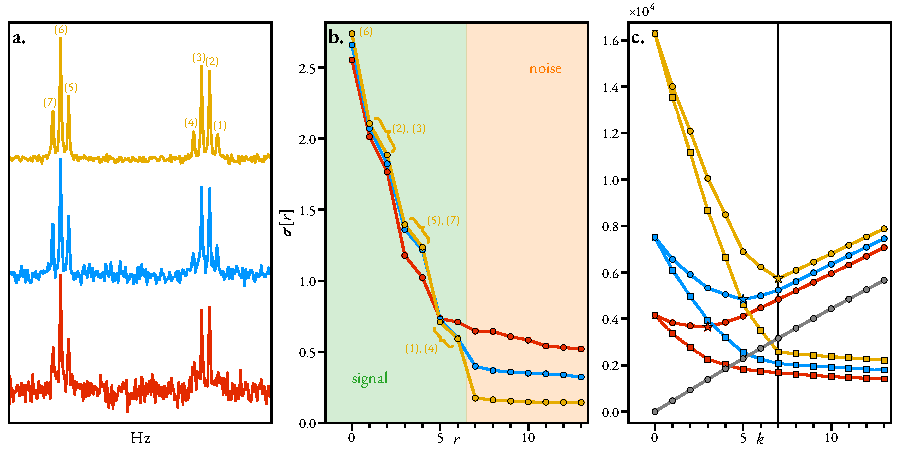
\includegraphics{mdl/mdl.pdf}
    \caption[
        A visualisation of the behaviour of the \acs{MDL} for three different
        \acsp{FID} comprising the same deterministic component, but with
        different noise variances.
    ]{
        A visualisation of the behaviour of the \acs{MDL} for three different
        \acsp{FID} comprising the same deterministic component ($\bx$) but
        with different noise instances of differing variances. The model used
        to construct the \acp{FID} features 7
        signals. The three \acsp{SNR} used were
        \qty{7}{\deci\bel} (red), \qty{12}{\deci\bel} (blue), and
        \qty{20}{\deci\bel} (yellow). The \acsp{FID} were generated with $N
        = 256$.
        \textbf{a.} Spectra of the three \acsp{FID}.
        \textbf{b.} The values of the 14 most significant singular values
        associated with the Hankel matrix $\Hy$, with the
        pencil parameter $L$ set to $\lfloor \nicefrac{N}{3} \rfloor =
        85$.
        \textbf{c.} Square points with dotted lines: The negative log-likeliood
        at the \ac{MLE}, i.e. the first term of \cref{eq:mdl}.
        Grey line: the penalty component of the \ac{MDL}, given by the second
        term in \cref{eq:mdl}.
        Circular points with solid lines: the \ac{MDL}.
        Stars denote the minimum of the \ac{MDL} for a given \ac{FID}. The
        \qty{20}{\deci\bel}
        signal is correctly deemed to have a model order of 7, while the other
        two are underestimated (predicted models orders are 5 and 3 for the
        \qty{12}{\deci\bel} and \qty{7}{\deci\bel} \acsp{FID}, respectively).
    }
    \label{fig:mdl}
\end{figure}
Applying the \ac{MDL} for model order selection, and subsequently using the
\ac{MPM} for parameter estimation is the basis of the \ac{ITMPM}\cite{Lin1997}.
\Cref{fig:mdl} illustrates the form of the \ac{MDL} for three signals
with equivalent underlying models, with $M=7$, and noise instances with
different variances. The first 14 singular values of $\Hy$
are plotted in panel b, where it can be seen that beyond the first 7,
which account for signal components, the subsequent singular values, decrease
at a far slower rate. The noise subspace for \acp{FID} with higher \acp{SNR}
have singular values which are (a) smaller in magnitude and (b) more
consistent, such that distinguishing the noise and signal subspaces is an
easier task (cf. the yellow and red lines in panel b). As such, the
\ac{MDL} is more likely to provide a faithful estimate of the true number of
components in the \ac{FID} (panel c) when the \ac{SNR} is higher.
